\documentclass[../../main.tex]{subfiles}

 \lhead{Implementation: Real RIR Measurements}
 
\begin{document}

\subsection{Real RIR Recordings}
\label{realRIRs}

	For testing the difference in perception of movement when using synthetic or real \ac{RIR}'s, real measurements were taken in Hendrix Hall.
	
%-------------RIR Setup-------------%
	\subsubsection{RIR Measurement Setup}

		For the \ac{VSS} it is desirable to obtain \ac{RIR}'s that can be used to represent the topology of a singer, i.e mouth (sound source) bellow the ears (receiver). To achieve this, a Genelec 8040B \cite{genelec} loudspeaker was used as a directional sound source and a Soundfield St450 MKII microphone \cite{st450} was used as the receiver to record the three dimensional sound field in Ambisonic B-format. 

		Figure~\ref{realRIRTop} shows an image of an approximate human head topology sound source and receiver set up. The Genelec is placed 1m above the ground (from the base of the speaker to the floor) and the Soundfield microphone placed 0.6m above the sound source. Ideally the receiver would be placed closer to the sound source to more accurately represent the distance between the ears and the mouth, however due to the physical dimensions of the equipment being used this was not possible. The sound source was placed 1m off the ground simply due to the limitations set by the maximum height of the microphone stand.

			%-------------Topology Image-------------%
		\begin{figure}[H]
			\begin{center}
				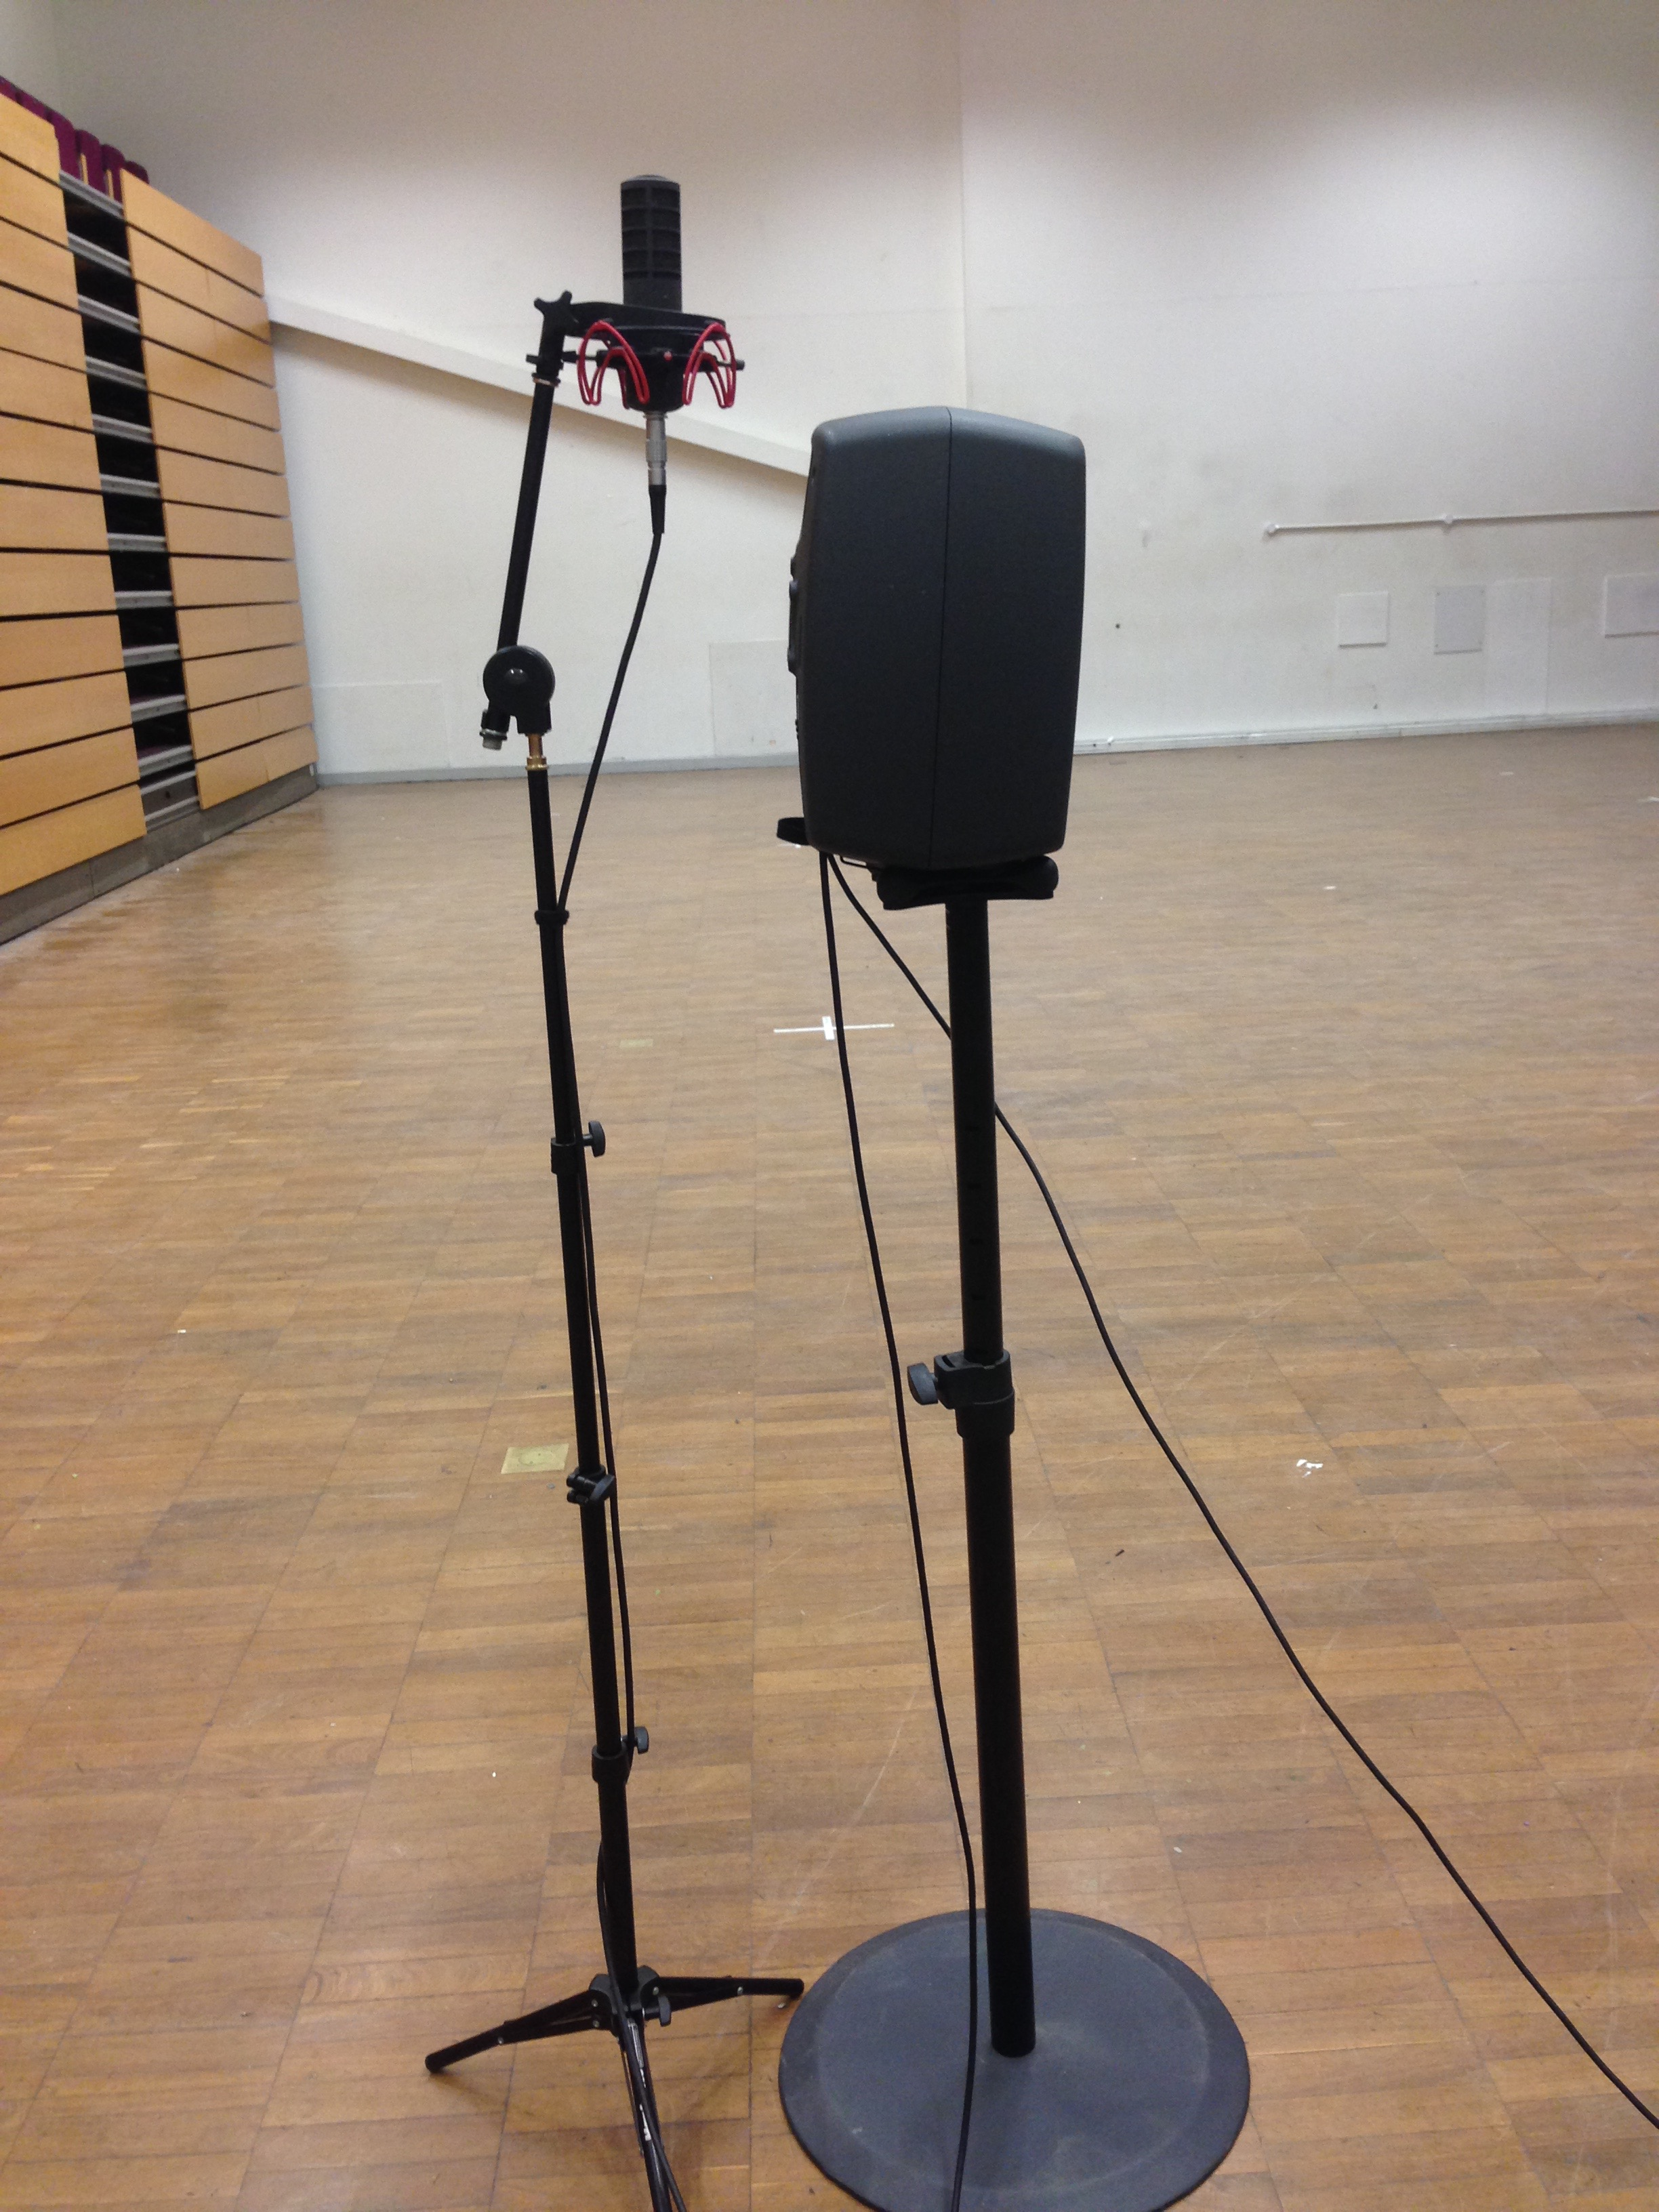
\includegraphics[scale = 0.06]{Sections/Implementation/RealRIRs/images/realRIRTopology1.jpg} 
				\caption{Human head topology \ac{RIR} measurement set up with a Genelec 8040B sound source placed 1m off the floor 0.6m below a Soundfield microphone used as a receiver.}
				\label{realRIRTop}
			\end{center}
		\end{figure}

		%Figure~\ref{realRIRSetup} shows the overall set up used for recording the \ac{RIR}'s as follows: \textbf{(1)} the Genelec and Soundfield microphone in the above mentioned source and receiver set up with a special soundfield cable running into \textbf{(2)}, the soundfield unit used to output an Ambisonic B-format signal through 4 XLR to jack cables to \textbf{(3)} a Fireface UXC audio interface plugged into \textbf{(4)} a Mac running the digital audio workstation Reaper. Reaper was used to record directly to a single 4 channel track where channels 1 - 4 recorded the W, X, Y, Z channels respectively, simultaneously output a 15 second long sinusoidal sweep to the Genelec. This method avoided synchronisation issues often faced when using separate devices to output a signal and to record a signal.

		Figure~\ref{realRIRSetup} shows the overall set up used for recording the \ac{RIR}'s as follows: \textbf{(1)} the Genelec and Soundfield microphone in the above mentioned source and receiver set up with a special soundfield cable running into \textbf{(2)}, the soundfield unit used to output an Ambisonic B-format signal through 4 XLR to jack cables to \textbf{(3)} a Fireface UXC audio interface plugged into \textbf{(4)} a Mac running the digital audio workstation Reaper.

		Reaper was used to:

		\begin{enumerate}
		 \item Record directly to a single 4 channel track where channels 1 - 4 recorded the W, X, Y, Z channels respectively
		 \item Output a 15 second long sinusoidal sweep to the Genelec.
		 \end{enumerate}

		 Using reaper to do both simultaneously avoided synchronisation issues often faced when using separate devices to output and record a signal.

		%-------------Setup-------------%
		\begin{figure}[H]
			\begin{center}
				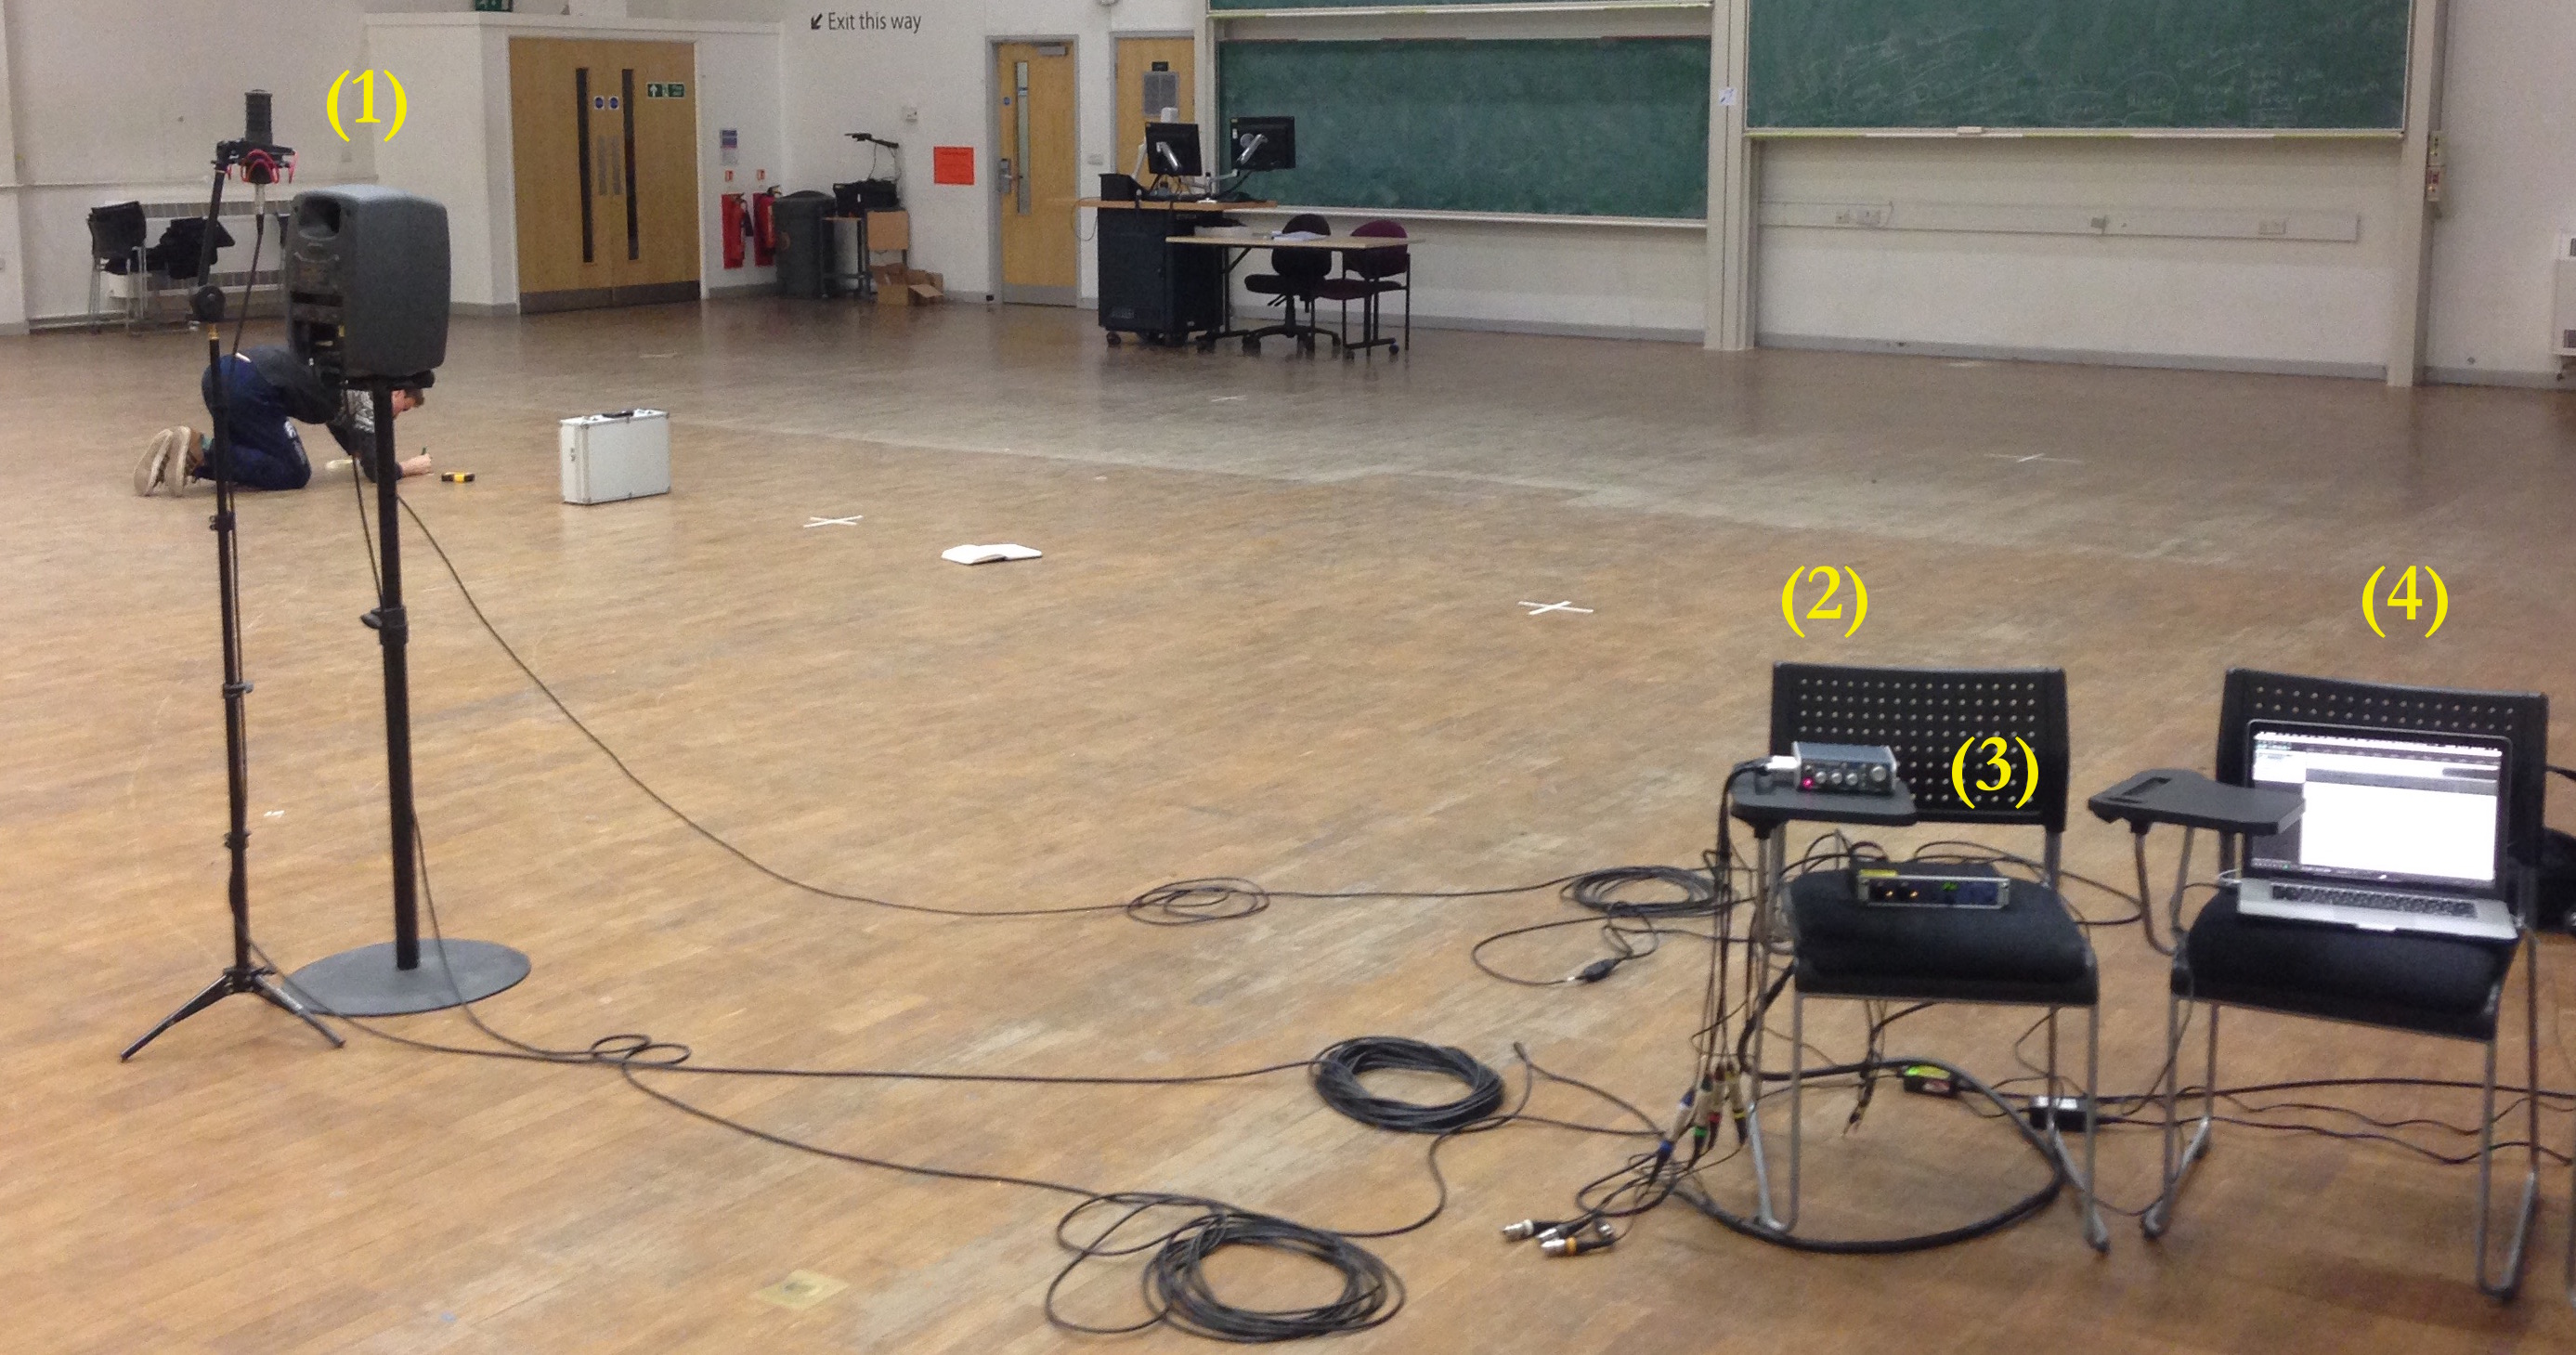
\includegraphics[scale = 0.14]{Sections/Implementation/RealRIRs/images/realRIRSetup_edit.jpg} 
				\caption{Real \ac{RIR} measurement set up. \textbf{(1)}: Sound source and receiver set up \textbf{(2)}: Soundfield interface \textbf{(3)}: Fireface UXC audio interface \textbf{(4)}: Mac running Reaper to output sinusoidal sweep and record B-format input.}
				\label{realRIRSetup}
			\end{center}
		\end{figure}

	%-------------Positions-------------%
	\subsubsection{Positions}

		Four positions within the room were chosen and marked with tape for the \ac{RIR} positions shown in figure~\ref{rirPositions} where:

		\begin{center}
			\begin{tabular}{l| c c c c}
				Position & (1) & (2) & (3) & (4) \\
			Coordinates [x(m), y(m)] & [9,9] & [4.5,9] & [2,9] &  [10.13,1.46]\\
			\end{tabular}
		\end{center}

		\vspace{5mm}


		For each position, an \ac{RIR} was taken in four different directions. Starting at 0\textdegree~, the sound source was rotated anti-clockwise in 90\textdegree~increments (anti-clockwise rotation is a standard in Ambisonics). Rotating the sound source and keeping the receiver at 0\textdegree (facing the blackboards) ensures that when the user turns their head in the \ac{VSS} the sound field does not rotate as they do. Once the four directional \ac{RIR} were recorded, the source and receiver were moved to the next marked location with care being taken to make sure the receiver is placed the same distance away from the sound source each time.

		%-------------Real RIR Positions Image-------------%
		\begin{figure}[H]
			\begin{center}
				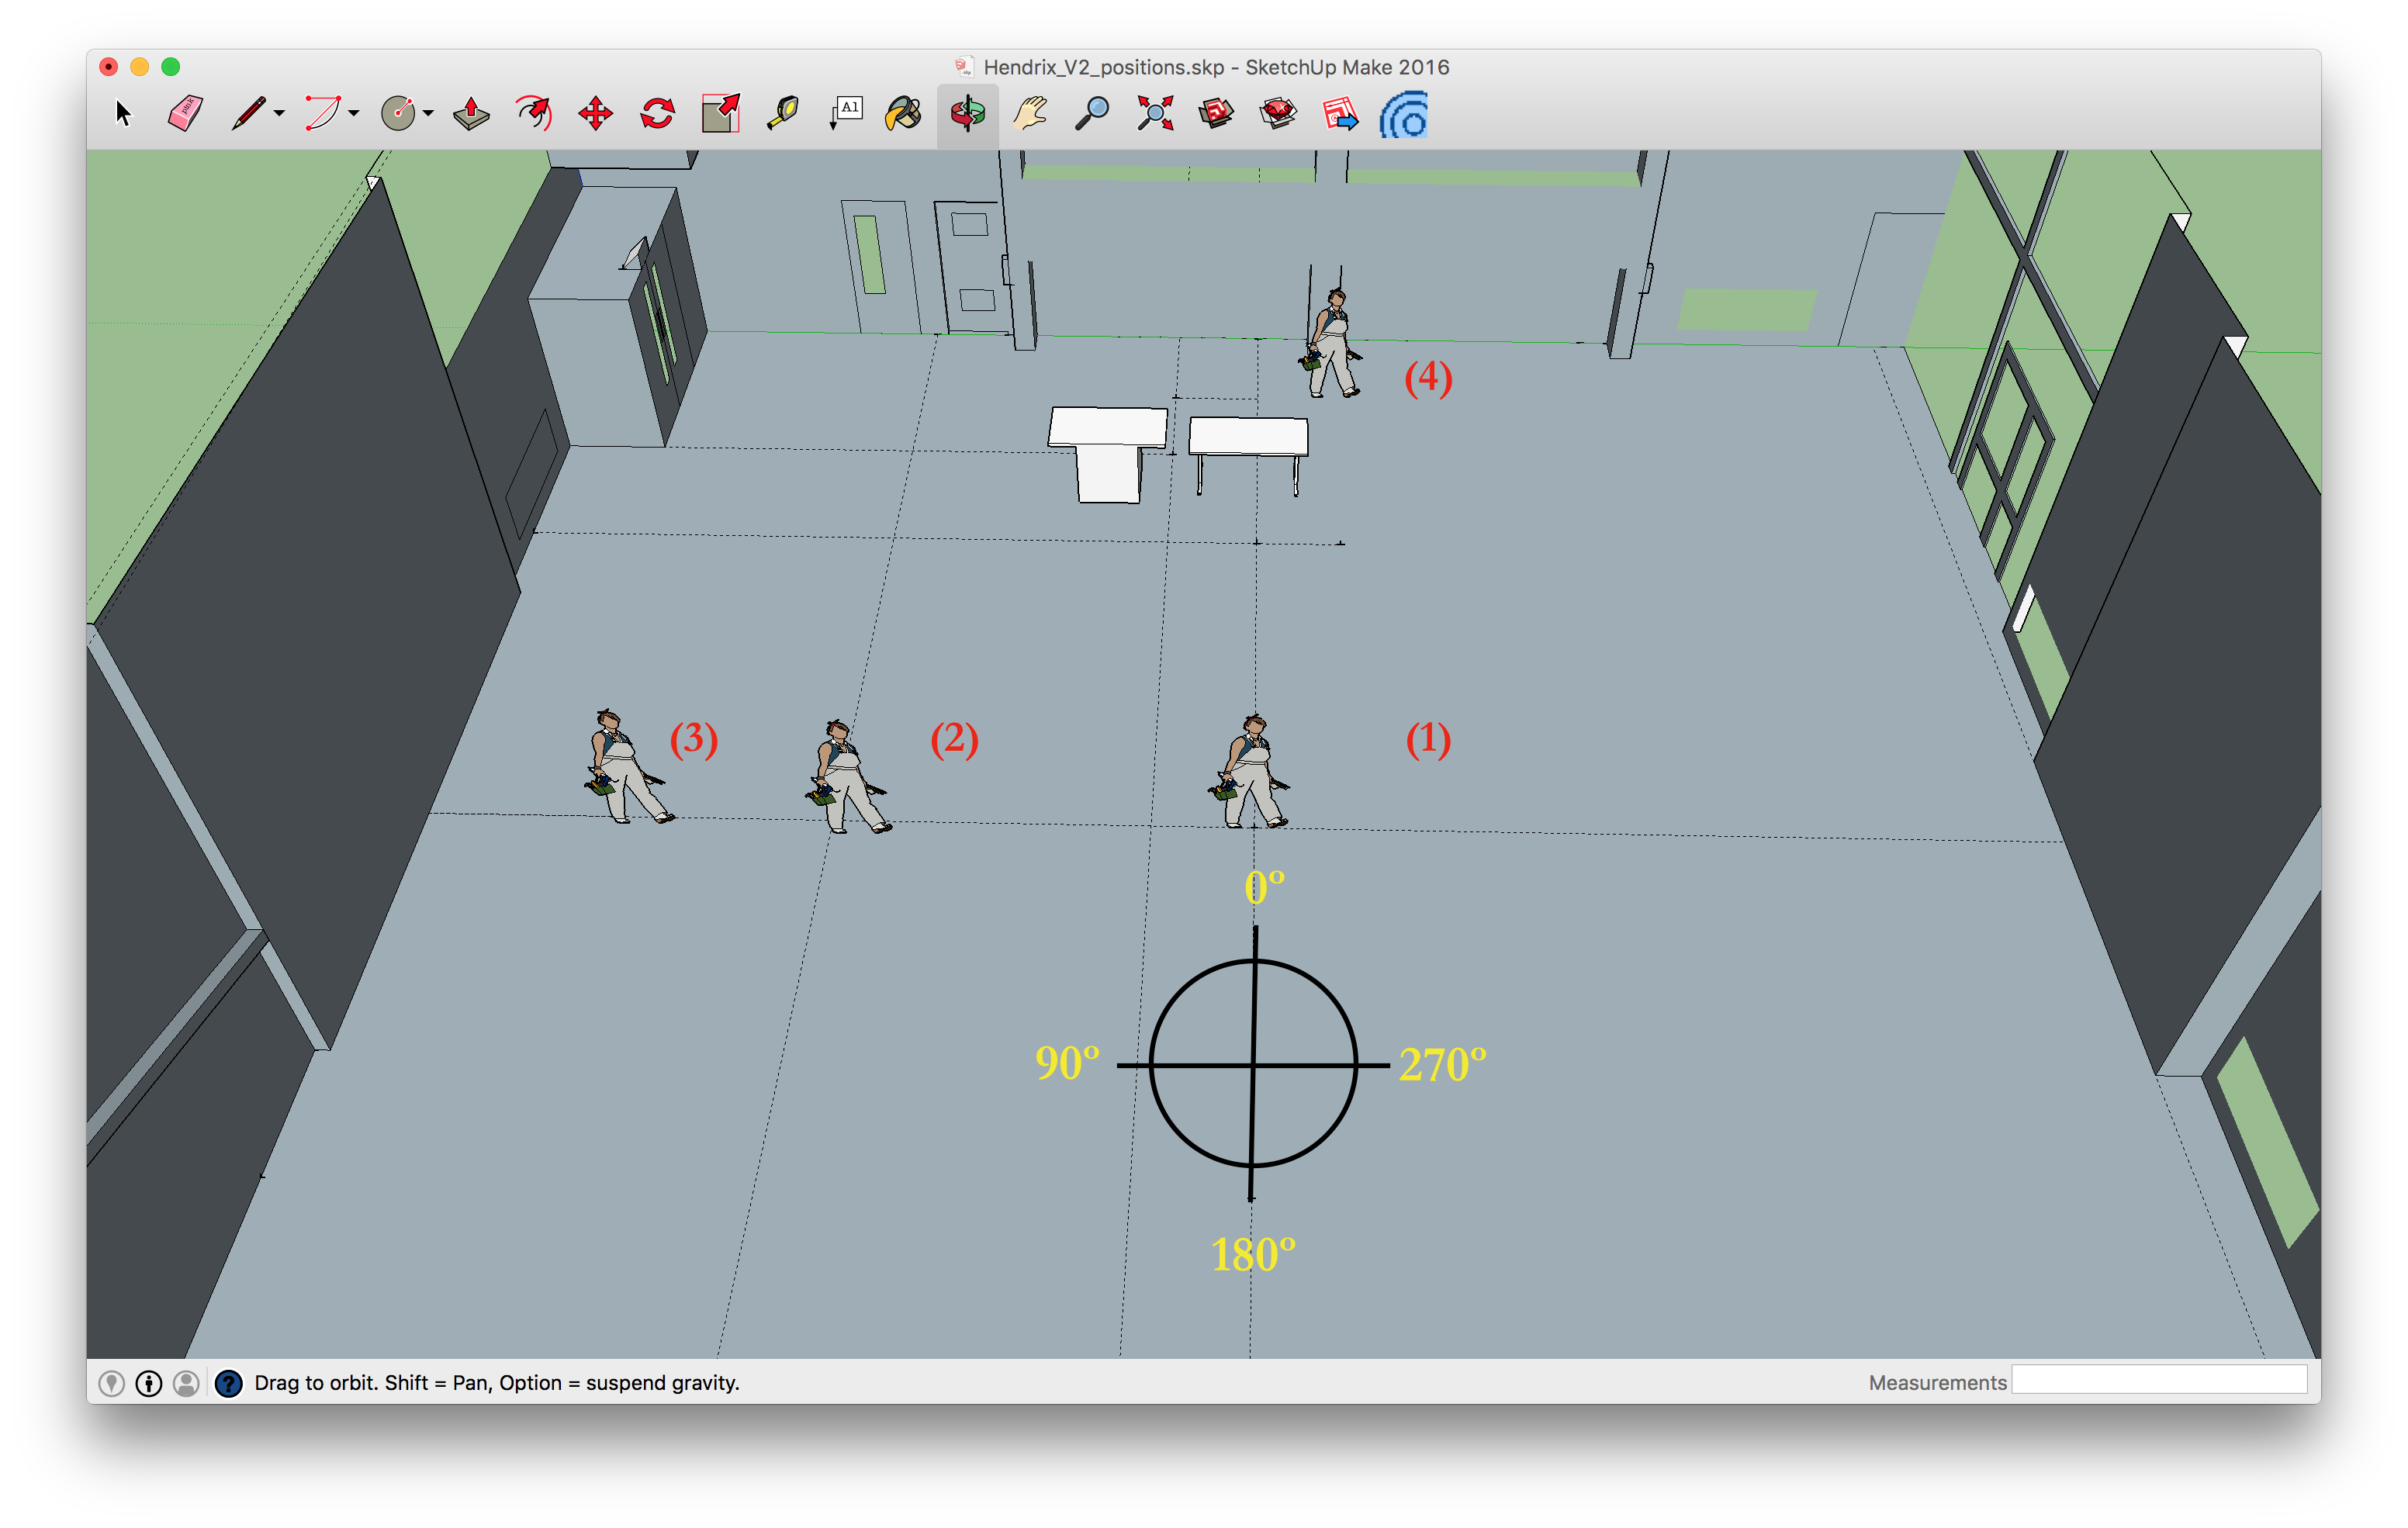
\includegraphics[scale = 0.3]{Sections/Implementation/RealRIRs/images/Real_RIRs7_editV2.png} 
				\caption{Google SketchUp model showing the positions of where the real \ac{RIR}'s were taken. The compass shows 0\textdegree facing what has been defined as the front of the room.}
				\label{rirPositions}
			\end{center}
		\end{figure}
		% \begin{figure}[ht]
		% 	\begin{center}
		% 		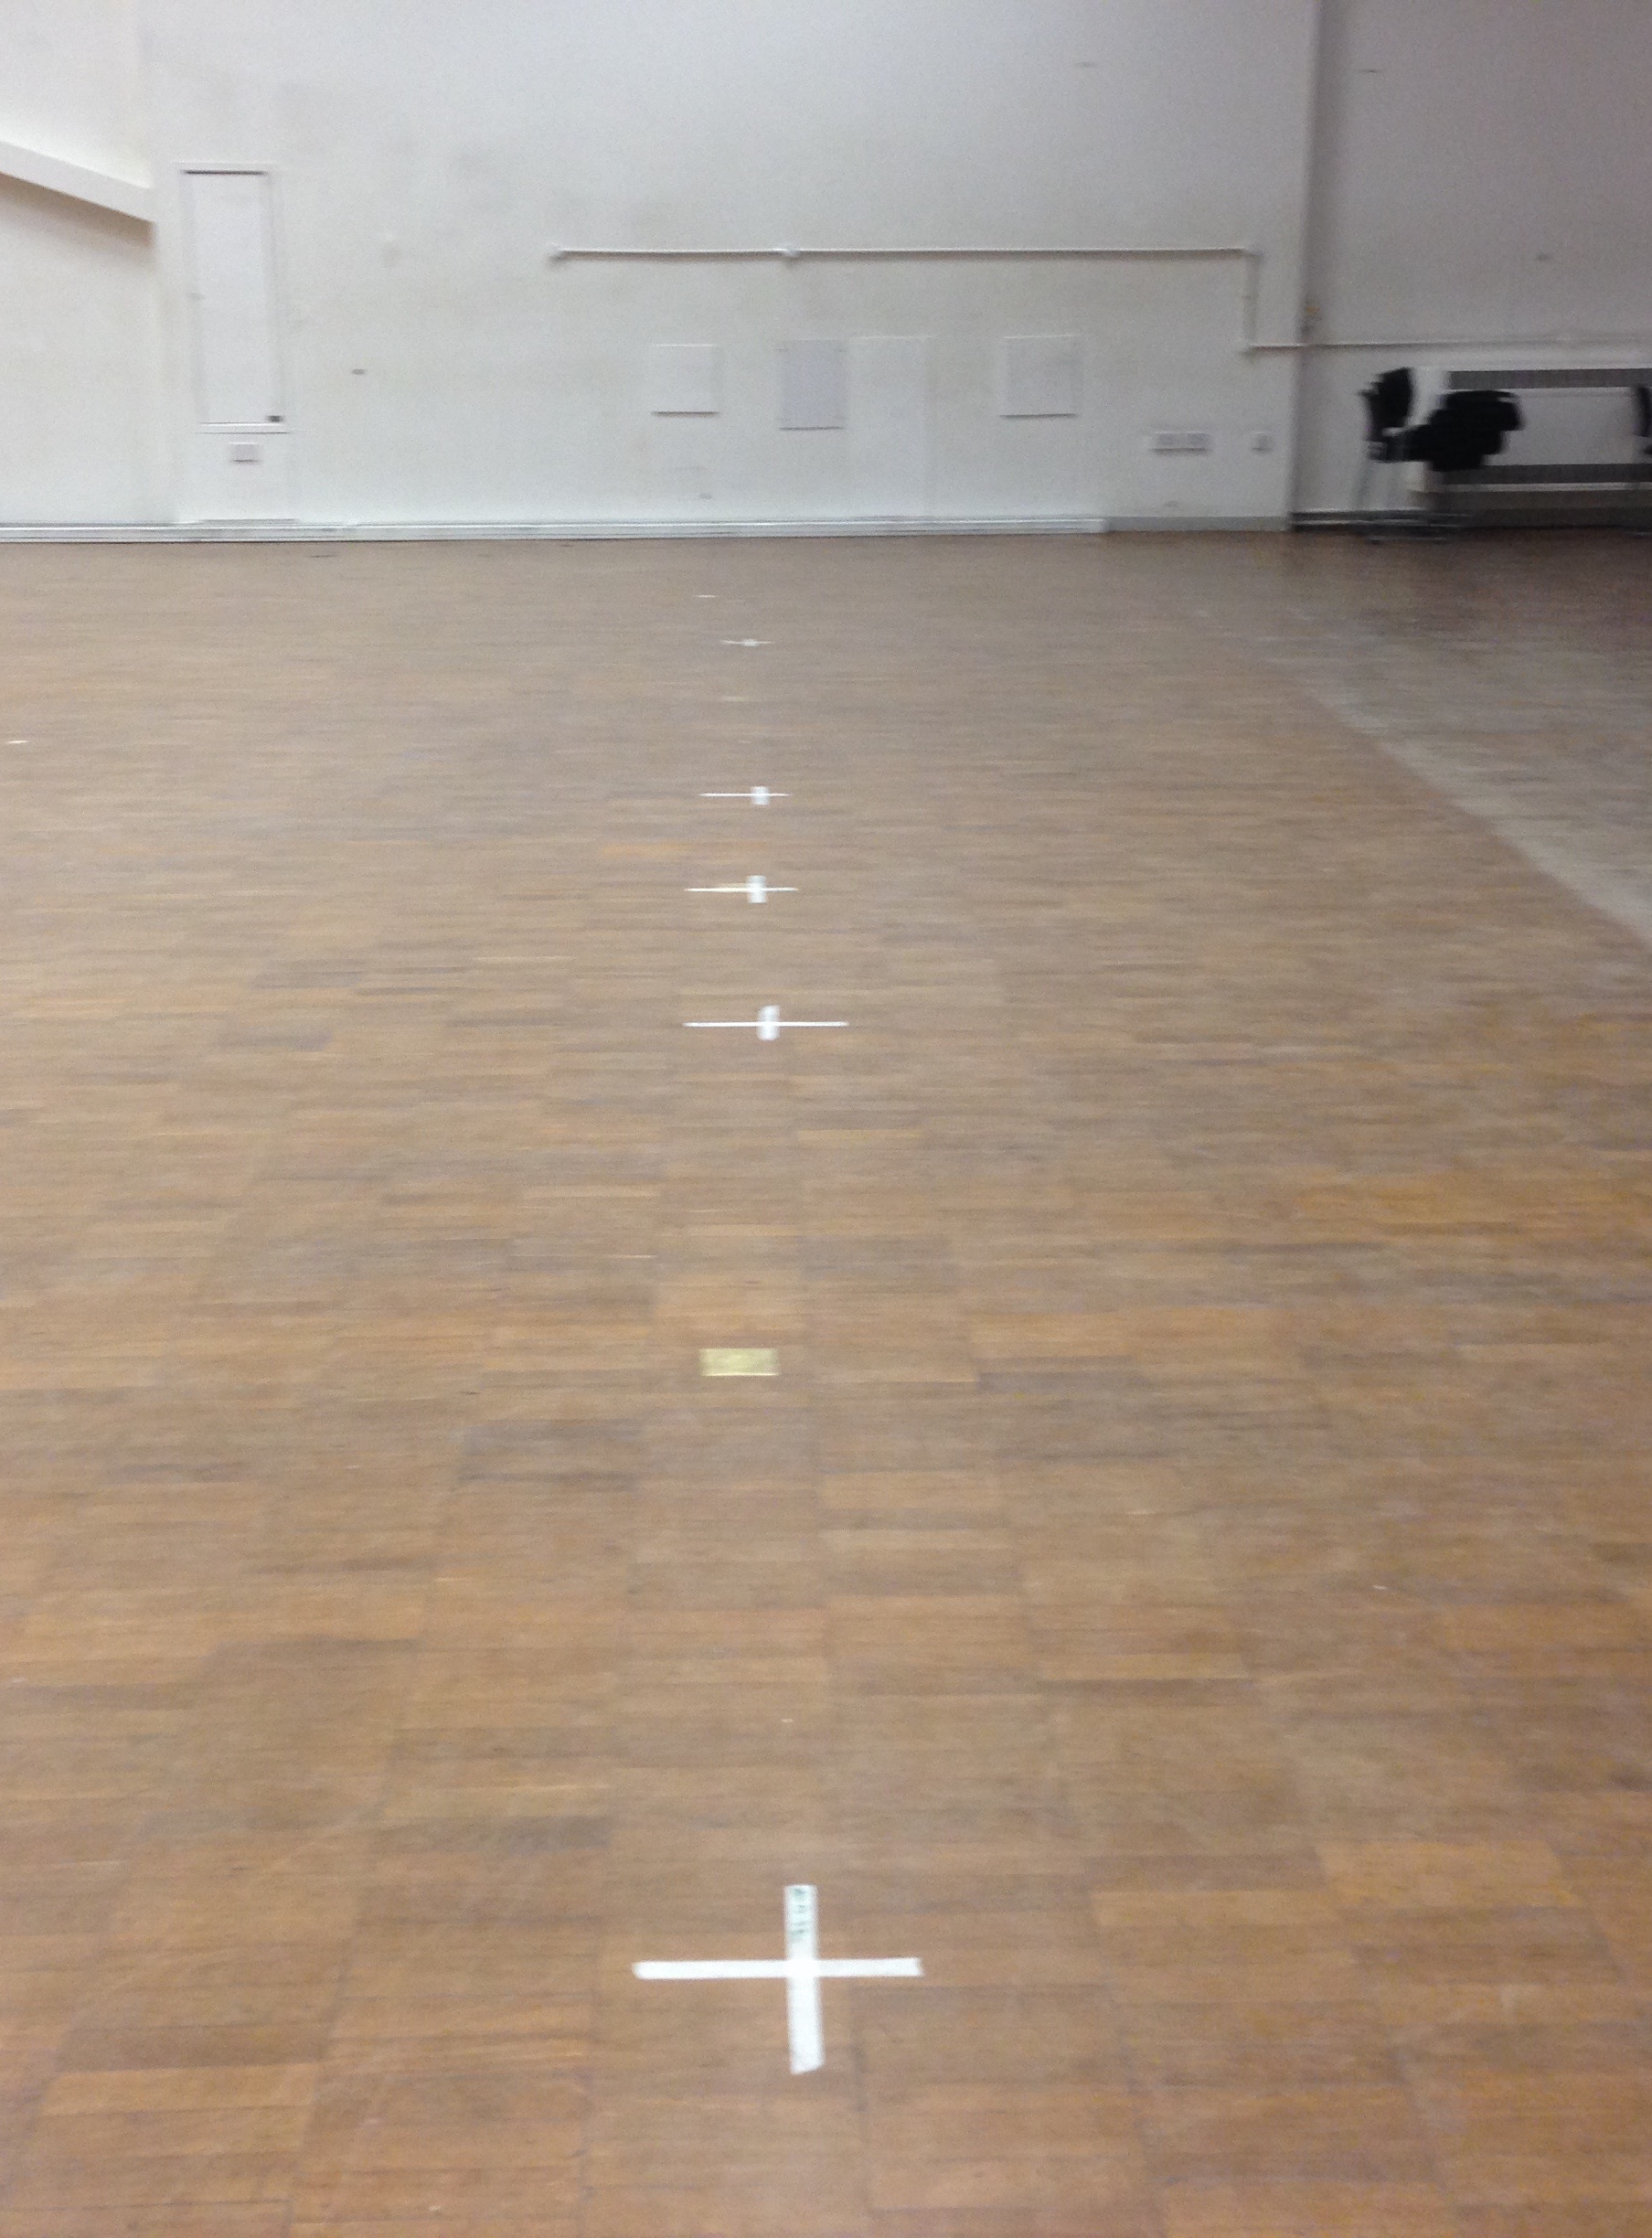
\includegraphics[scale = 0.15]{Sections/Implementation/RealRIRs/images/realRIRTape_edit.jpg} 
		% 		\caption{Google SketchUp model showing the positions of where the real \ac{RIR}'s were taken}
		% 		\label{rirPositions}
		% 	\end{center}
		% \end{figure}

	%-------------Measurements-------------%
	\subsubsection{Measurements}
		The sound source signal used was a 15 second long exponentially swept sinusoid ranging from 20Hz to 20kHz with an 8 second padding to ensure that the room could be vacated before the sweep began. The sweep was produced using the Matlab function \href{http://lt669.github.io/code/matlab/html/generatesweep.html}{\texttt{generatesweep.m}} taken from the departmental website \cite{sineSweep} which produced both the sinusoidal sweep and an inverse sinusoidal sweep used for deconvolution at a later stage.
		
	\subsubsection{Measurements Post-Production}

		Once the measurements had been recorded, the first 8 seconds of the files were muted in order to remove noise such as door slams as the room was vacated. Then the signals were deconvolved with an inverse of the sinusoidal sweep to time align the frequency dependant room reflections. This was done using the deconvolution Matlab function \href{http://lt669.github.io/code/matlab/html/deconvolve.html}{\texttt{deconvolve.m}} taken from the departmental website \cite{sineSweep}.

	\subsubsection{Issues}
		Several issues arose when taking the initial \ac{RIR}'s. Simply connection the outputs from the Soundfield converter to the incorrect inputs on the Fireface audio interface meant that the initial recordings contained tracks that were not necessarily recorded in the correct order, i.e the tracks were not recorded as [W, X, Y, Z] but could have been recorded in a possible 24 combinations. This meant that when used to convolve with an audio source, the localisation of the sound source would be incorrect.


		In an attempt to salvage the potentially ruined \ac{RIR} recordings, the tracks were analysed through observation and convolution with test tracks. However, though it was possible to narrow down which order the channels might have been recorded in, pinpointing the track order could not be done with 100\% accuracy. Therefore, Hendrix Hall was rebooked and the measurements were taken again.



%--------------------------Link Testing--------------------------%
% There a link like: \href{/SuportingFiles/doc.pdf}{Audio!}

% \href{file:/SuportingFiles/index.html}{Fuck it}

% \href{run:/SuportingFiles/.}{DirectoryFUCK}

% \HREF{run:/SuportingFiles/.}{Directory}

% \href{file:/SuportingFiles/CalMan_RIR.png}{Image}

\end{document}